% для компиляции в lualatex!!
%\documentclass[12pt, a4paper]{article}
\documentclass[12pt, a4paper]{disser}
\usepackage[english,russian]{babel}
\usepackage[warn]{mathtext}
%\usepackage[T2A]{fontenc}
%\usepackage[utf8]{inputenc}

\usepackage{xecyr} % Продукт Вашего покорного слуги ;)

%\setmainfont{DejaVu Serif}
\setmainfont{Liberation Serif}

\usepackage{color}
\usepackage{amssymb,amsmath}
\usepackage{graphicx}
\usepackage{multicol}

\textheight=24cm           % высота текста
\textwidth=16cm            % ширина текста
\oddsidemargin=0pt         % отступ от левого края
\topmargin=-1.5cm          % отступ от верхнего края
\parindent=24pt            % абзацный отступ
\parskip=0pt               % интервал между абзацами
\tolerance=2000            % терпимость к "жидким" строкам
\flushbottom               % выравнивание высоты страниц
%\def\baselinestretch{1.5} % печать с большим интервалом

%\title{}
%\author{\copyright~~С.А.~Назарова \thanks{e-mail:~sophia.nazarova@gmail.com}}
%\date{}


\begin{document}

	\begin{figure}[ht]
	
	\begin{minipage}[b]{.46\linewidth}
	%Фигурка в первом ряду слева размер отведенный под весь этот объект \textendash 0.46 от ширины строки
	%Параметр [b] означает, что выравнивание этих министраниц будет по нижнему краю
	\begin{center}
	{\tiny N Estuary Goreliy 1992 2012}
		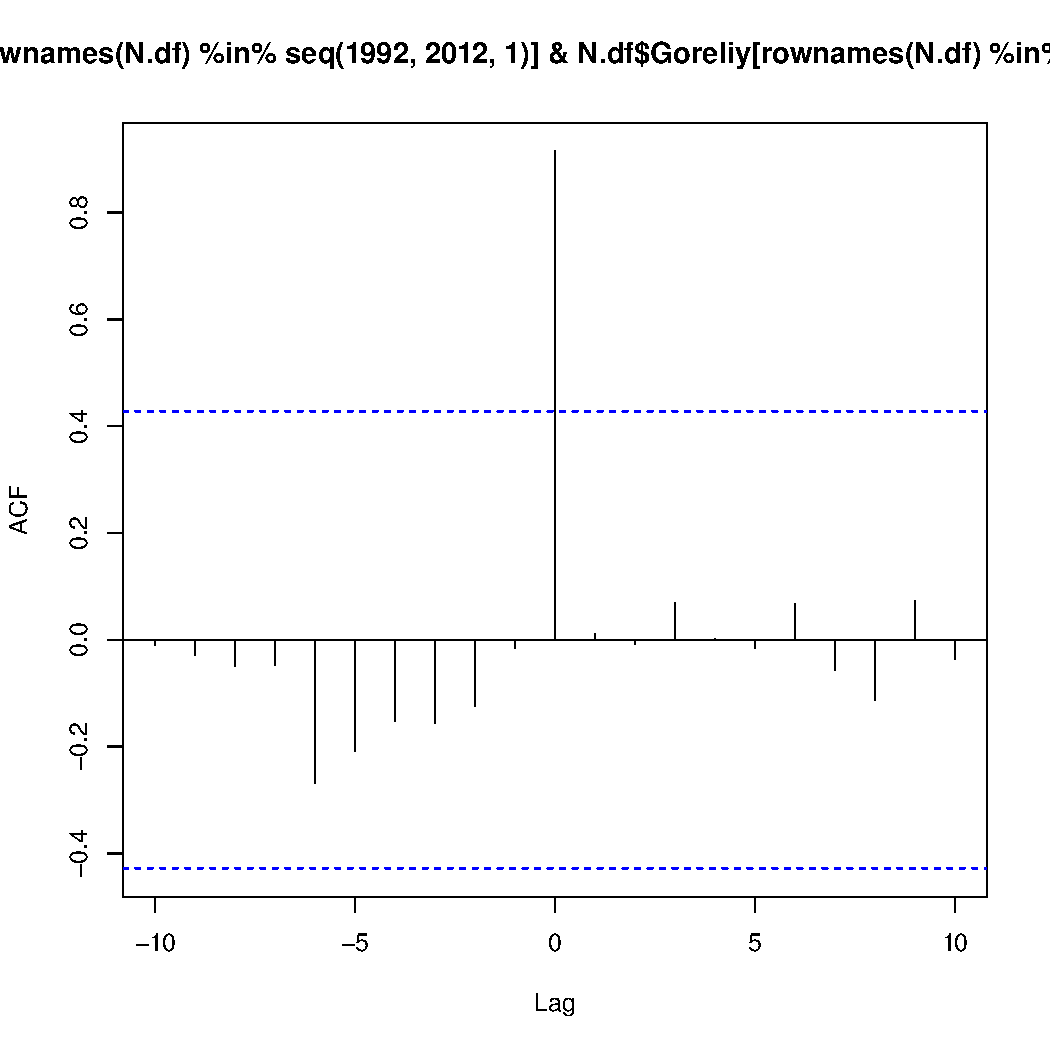
\includegraphics[width=65mm]{../White_Sea/dynamic_N_N1/crosscorr_N_Estury_Goreliy_1992_2012.pdf}

	\end{center}
	\end{minipage}
	%
	\hfil %Это пружинка отодвигающая рисунки друг от друга
	%
	\begin{minipage}[b]{.46\linewidth}
%Следующий рисунок - первый ряд справа %DUNGEON S_4 \ AB
	\begin{center}
	{\tiny N Estury Seldyanaya 1992 2012}
		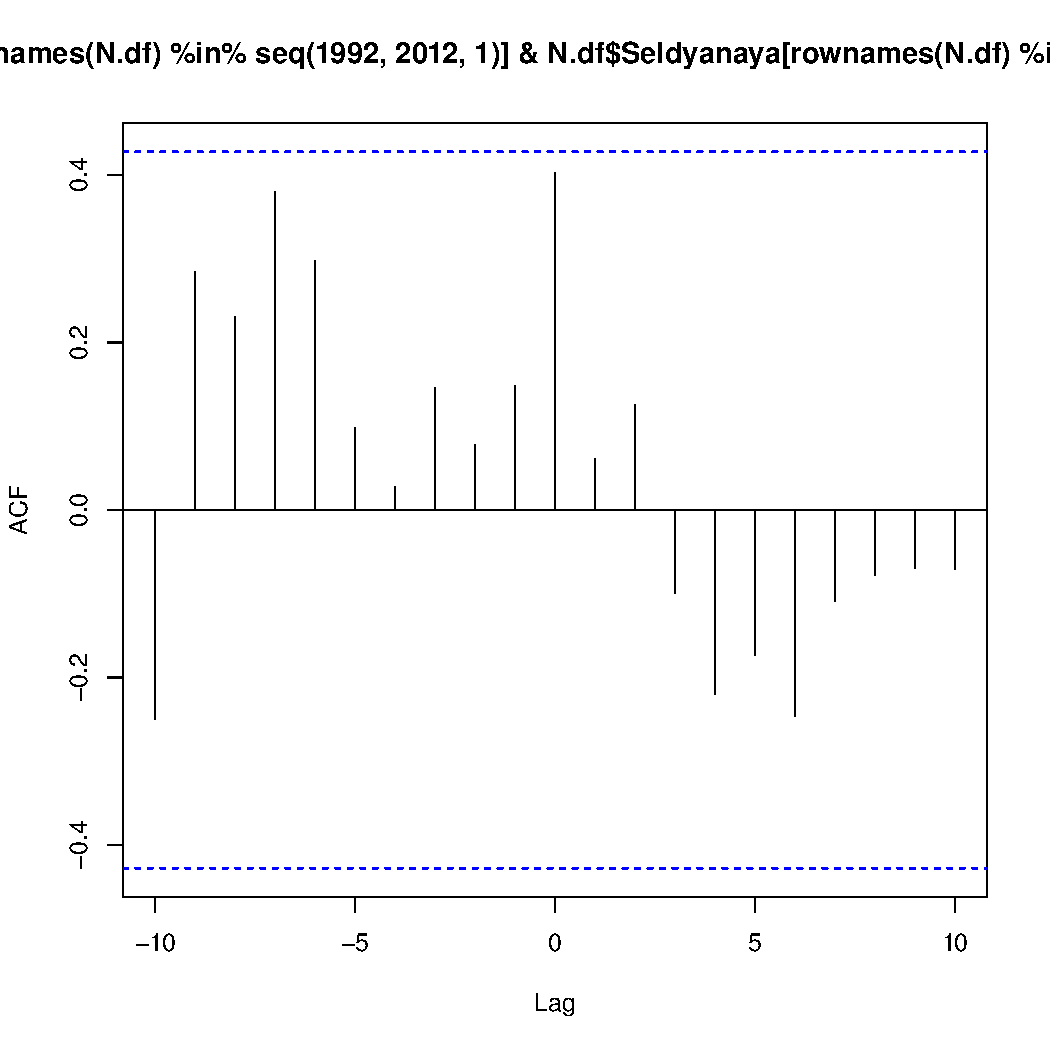
\includegraphics[width=65mm]{../White_Sea/dynamic_N_N1/crosscorr_N_Estury_Seldyanaya_1992_2012.pdf}
	\end{center}
	\end{minipage}

%\smallskip


	\begin{minipage}[b]{.46\linewidth}
%Фигурка в первом ряду слева размер отведенный под весь этот объект \textendash 0.46 от ширины строки
%Параметр [b] означает, что выравнивание этих министраниц будет по нижнему краю
	\begin{center}
	{\tiny N Estury Medvezhya 1992 2012}
	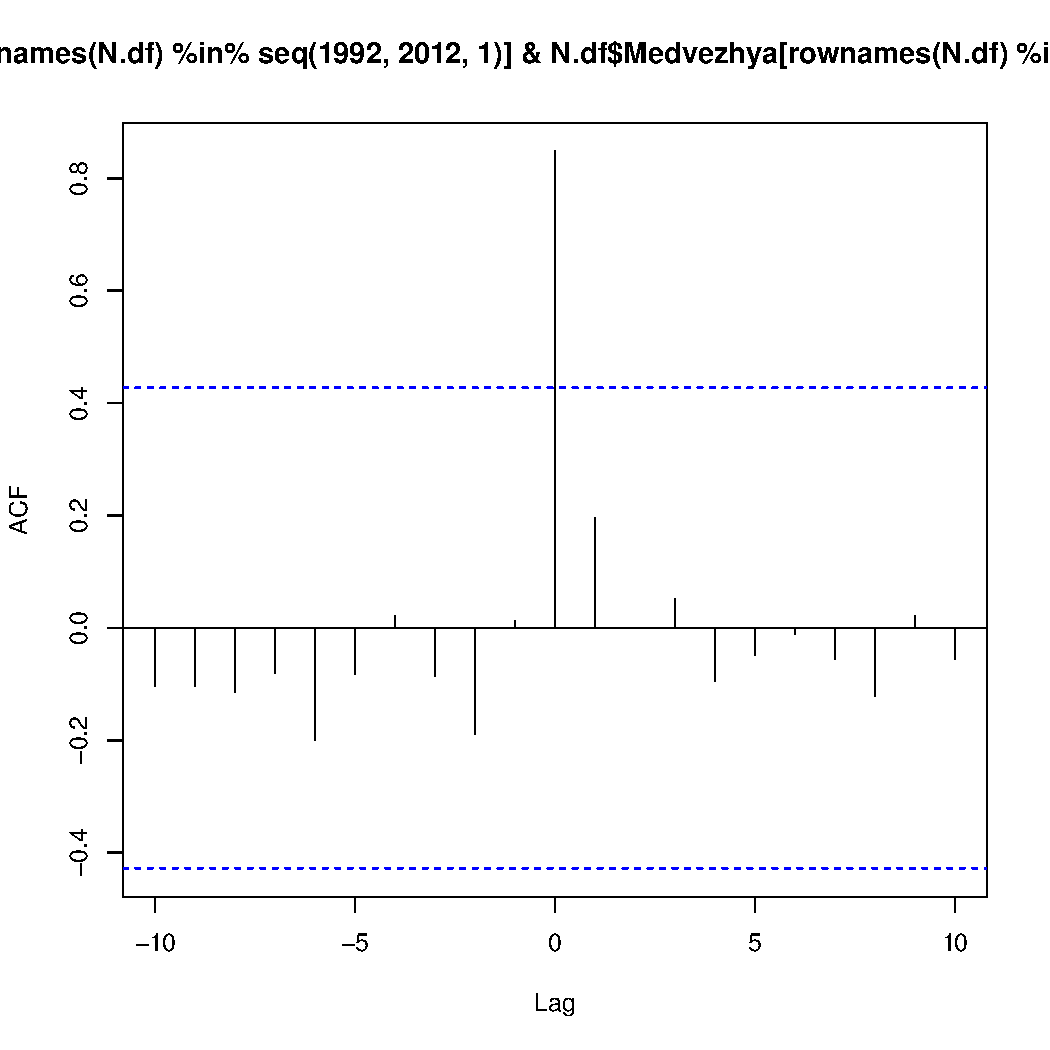
\includegraphics[width=65mm]{../White_Sea/dynamic_N_N1/crosscorr_N_Estury_Medvezhya_1992_2012.pdf}
	\end{center}
	\end{minipage}
%
	\hfil %Это пружинка отодвигающая рисунки друг от друга
%
	\begin{minipage}[b]{.46\linewidth}
%Следующий рисунок - первый ряд справа %DUNGEON S_4 \ AB
	\begin{center}	
	{\tiny  N Estury 2razrez 1992 2000}
	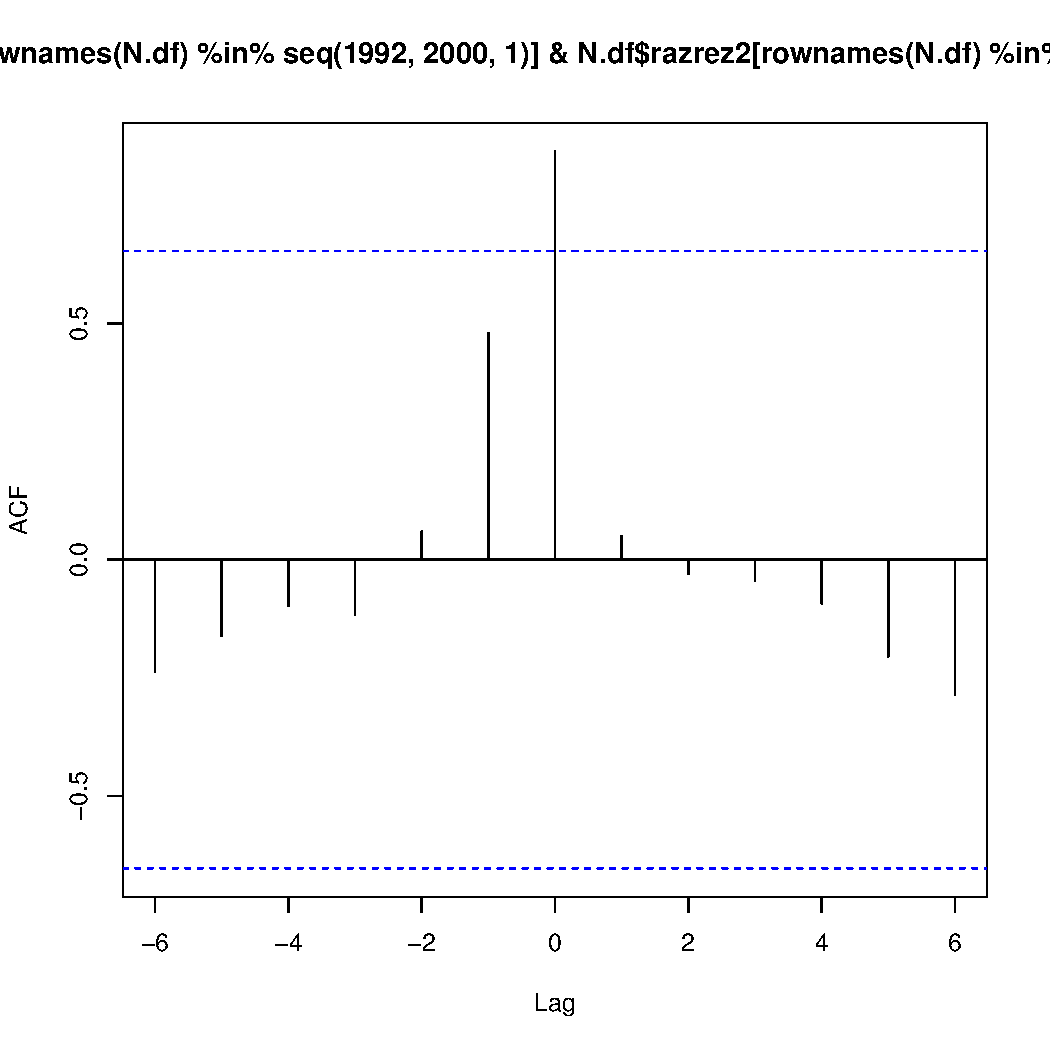
\includegraphics[width=65mm]{../White_Sea/dynamic_N_N1/crosscorr_N_Estury_2razrez_1992_2000.pdf}
	\end{center}
	\end{minipage}

%\smallskip

	\begin{minipage}[b]{.46\linewidth}
%Фигурка в первом ряду слева размер отведенный под весь этот объект \textendash 0.46 от ширины строки
%Параметр [b] означает, что выравнивание этих министраниц будет по нижнему краю
	\begin{center}
	{\tiny N Estury ZRS 1994 2012}
	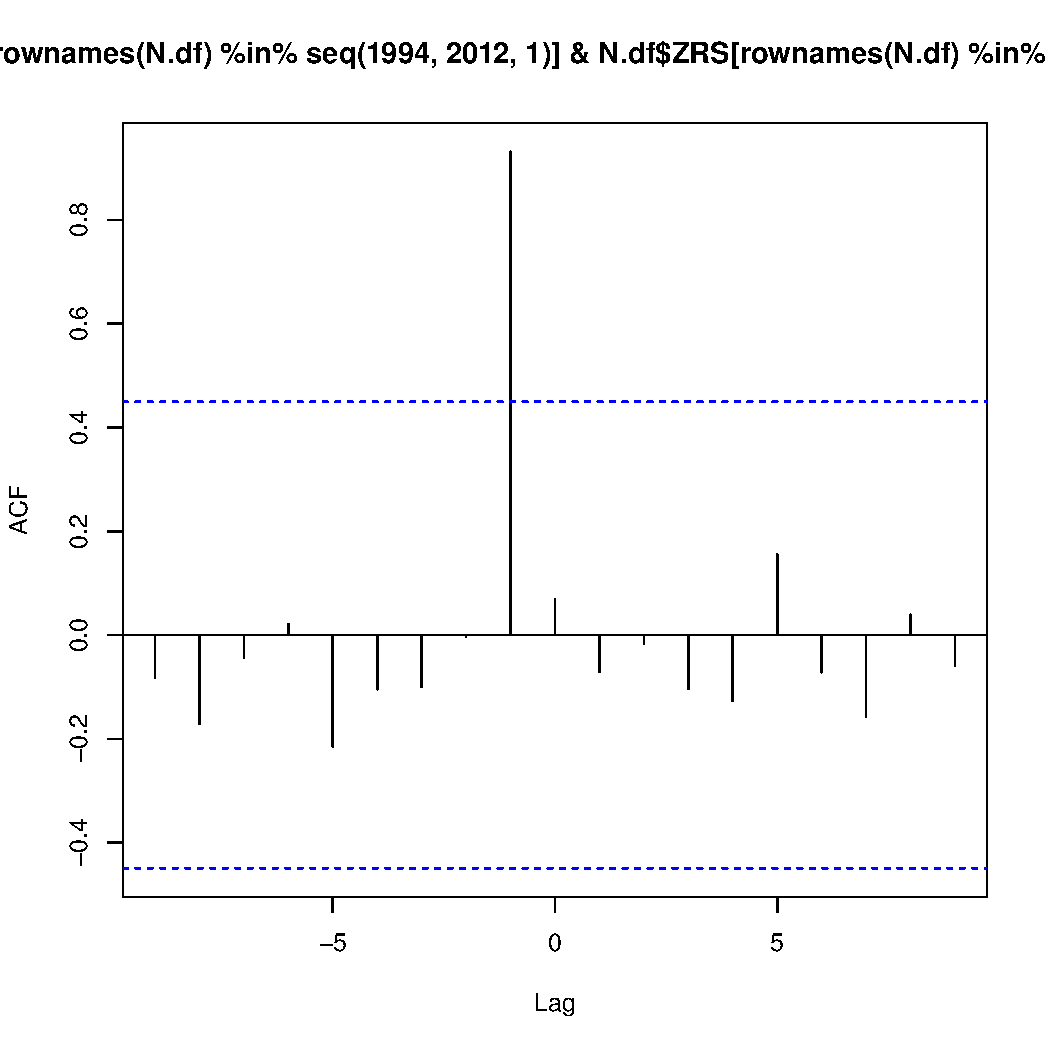
\includegraphics[width=65mm]{../White_Sea/dynamic_N_N1/crosscorr_N_Estury_ZRS_1994_2012.pdf}
	\end{center}
	\end{minipage}
%
	\hfil %Это пружинка отодвигающая рисунки друг от друга
%
	\begin{minipage}[b]{.46\linewidth}
%Следующий рисунок - первый ряд справа %DUNGEON S_4 \ AB
	\begin{center}
	{\tiny N Goreliy Seldyanaya 1992 2012}
	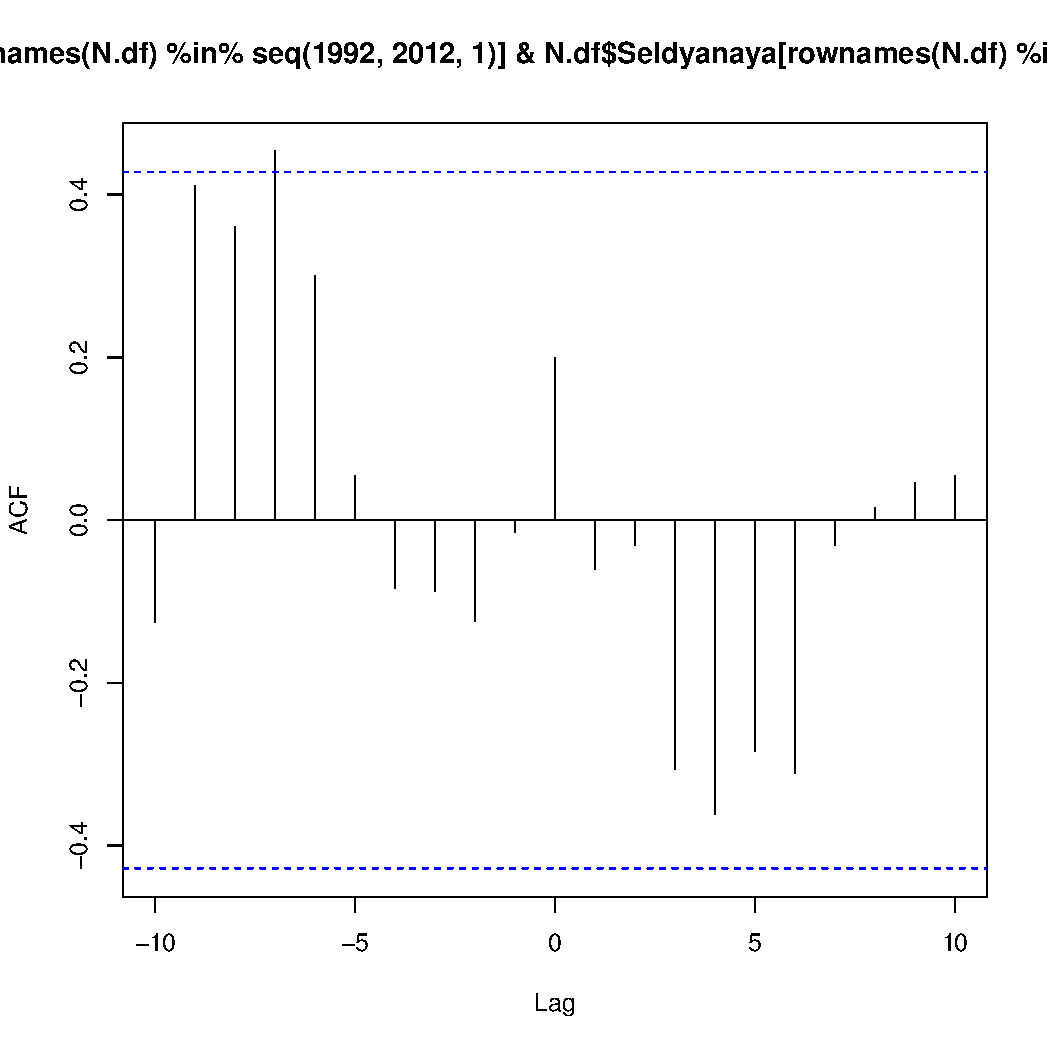
\includegraphics[width=65mm]{../White_Sea/dynamic_N_N1/crosscorr_N_Goreliy_Seldyanaya_1992_2012.pdf}
	\end{center}
	\end{minipage}

%\smallskip
	\caption{Кросскорреляции средней численности {\it Macoma balthica} на разных в Кандалакшском заливе}
	\label{ris:сcrosscorr_N_Kandalaksha}
	\end{figure}




	\begin{figure}[ht]
	
	\begin{minipage}[b]{.46\linewidth}
	%Фигурка в первом ряду слева размер отведенный под весь этот объект \textendash 0.46 от ширины строки
	%Параметр [b] означает, что выравнивание этих министраниц будет по нижнему краю
	\begin{center}
	{\tiny N Goreliy Medvezhya 1992 2012}
		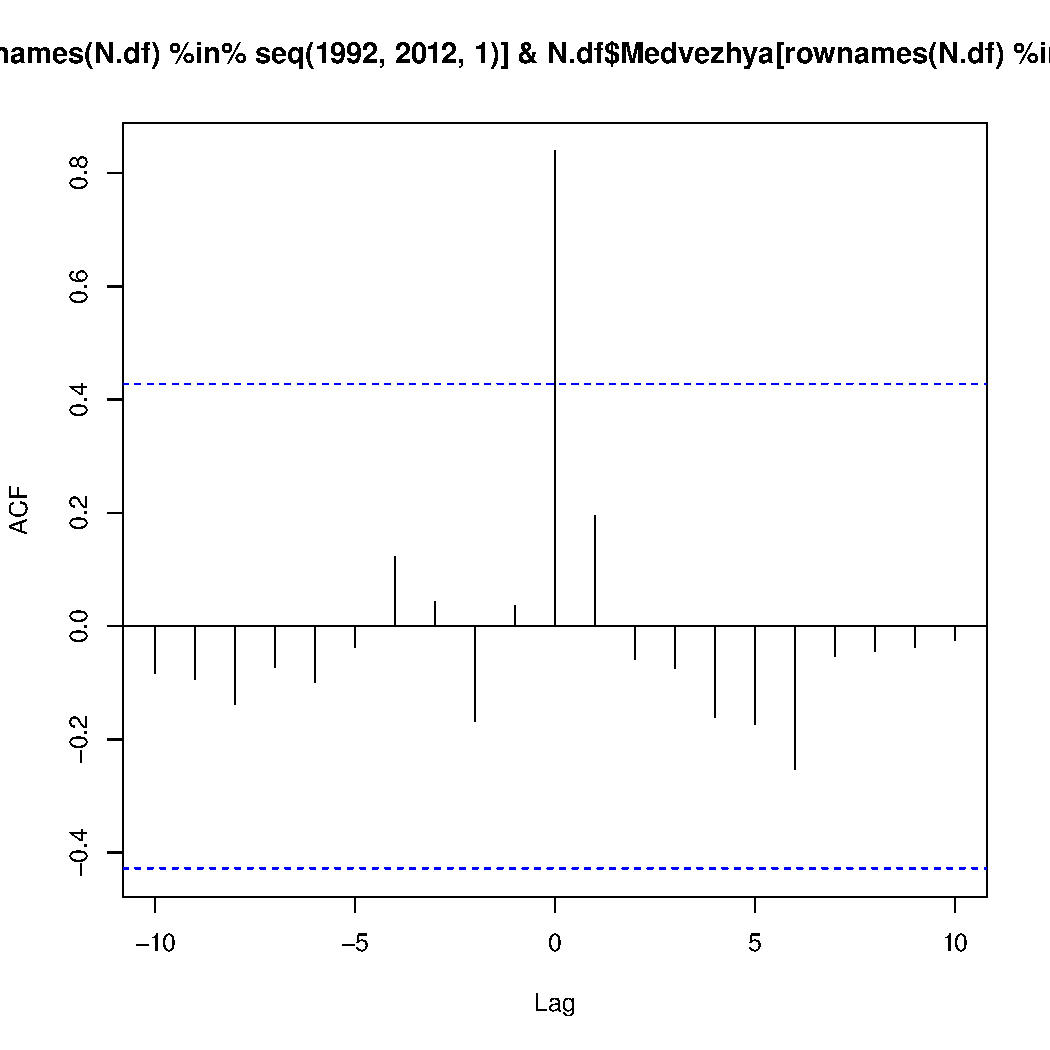
\includegraphics[width=65mm]{../White_Sea/dynamic_N_N1/crosscorr_N_Goreliy_Medvezhya_1992_2012.pdf}

	\end{center}
	\end{minipage}
	%
	\hfil %Это пружинка отодвигающая рисунки друг от друга
	%
	\begin{minipage}[b]{.46\linewidth}
%Следующий рисунок - первый ряд справа %DUNGEON S_4 \ AB
	\begin{center}
	{\tiny N Goreliy 2razrez 1992 2000}
		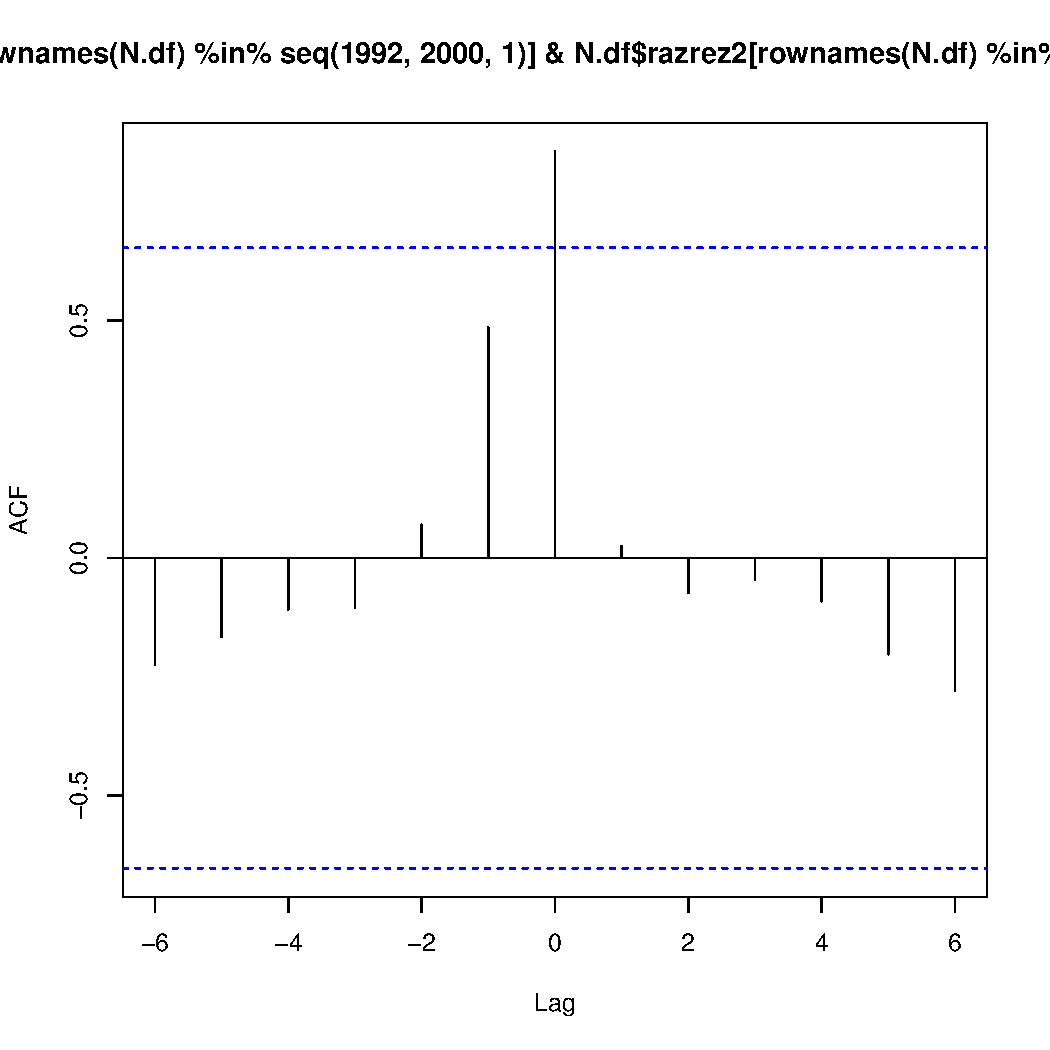
\includegraphics[width=65mm]{../White_Sea/dynamic_N_N1/crosscorr_N_Goreliy_2razrez_1992_2000.pdf}
	\end{center}
	\end{minipage}

%\smallskip


	\begin{minipage}[b]{.46\linewidth}
%Фигурка в первом ряду слева размер отведенный под весь этот объект \textendash 0.46 от ширины строки
%Параметр [b] означает, что выравнивание этих министраниц будет по нижнему краю
	\begin{center}
	{\tiny N Goreliy 2razrez 1992 2000}
	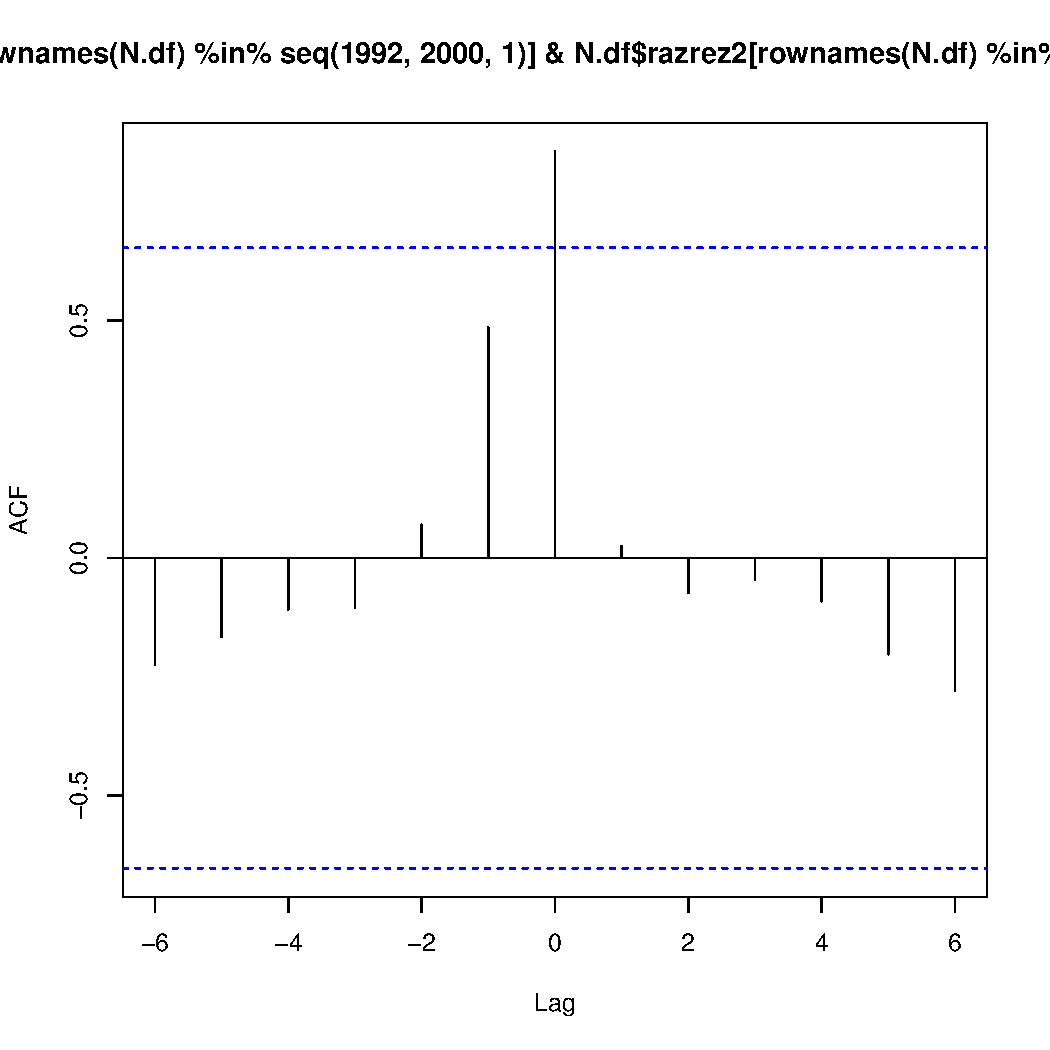
\includegraphics[width=65mm]{../White_Sea/dynamic_N_N1/crosscorr_N_Goreliy_2razrez_1992_2000.pdf}
	\end{center}
	\end{minipage}
%
	\hfil %Это пружинка отодвигающая рисунки друг от друга
%
	\begin{minipage}[b]{.46\linewidth}
%Следующий рисунок - первый ряд справа %DUNGEON S_4 \ AB
	\begin{center}	
	{\tiny N Goreliy ZRS 1994 2012}
	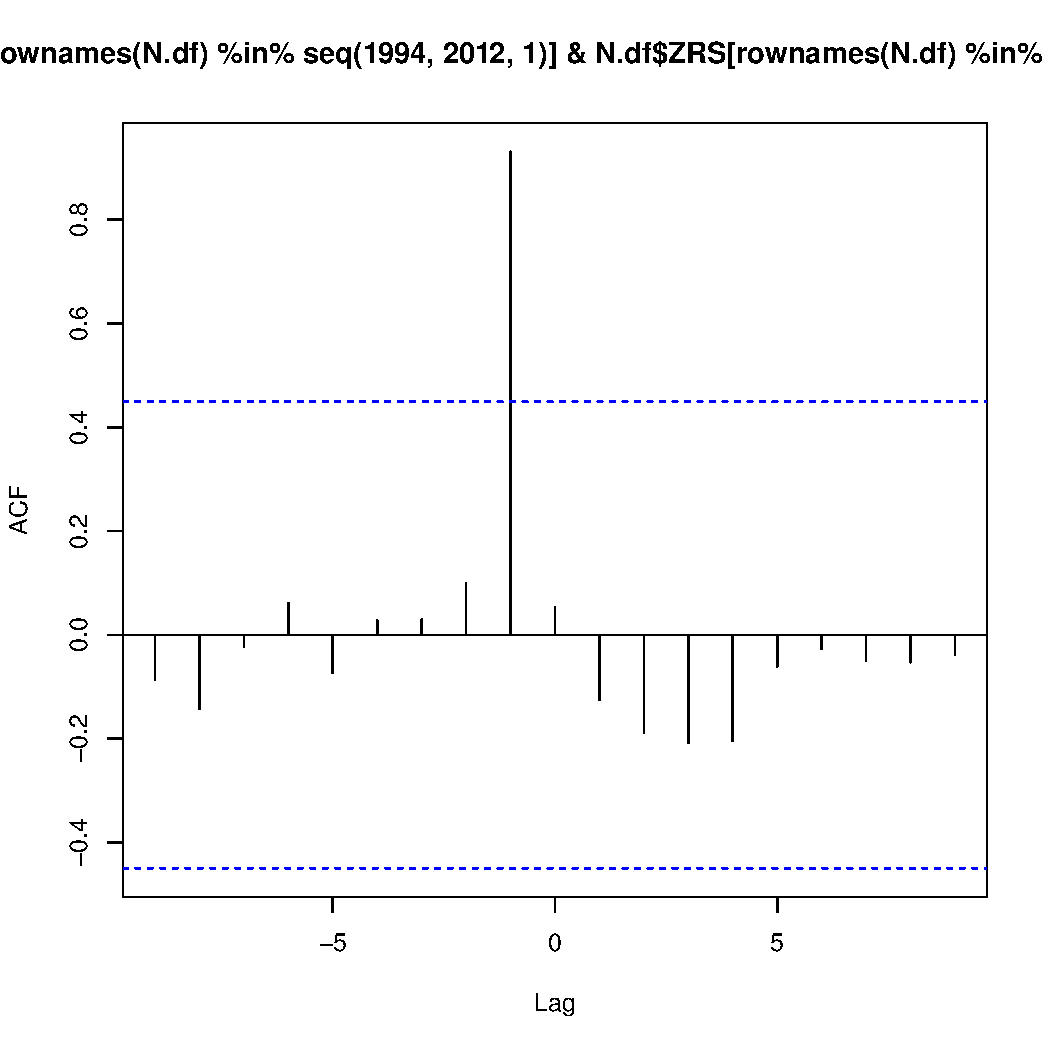
\includegraphics[width=65mm]{../White_Sea/dynamic_N_N1/crosscorr_N_Goreliy_ZRS_1994_2012.pdf}
	\end{center}
	\end{minipage}

%\smallskip

	\begin{minipage}[b]{.46\linewidth}
%Фигурка в первом ряду слева размер отведенный под весь этот объект \textendash 0.46 от ширины строки
%Параметр [b] означает, что выравнивание этих министраниц будет по нижнему краю
	\begin{center}
	{\tiny  N Seldyanaya 2razrez 1992 2000}
	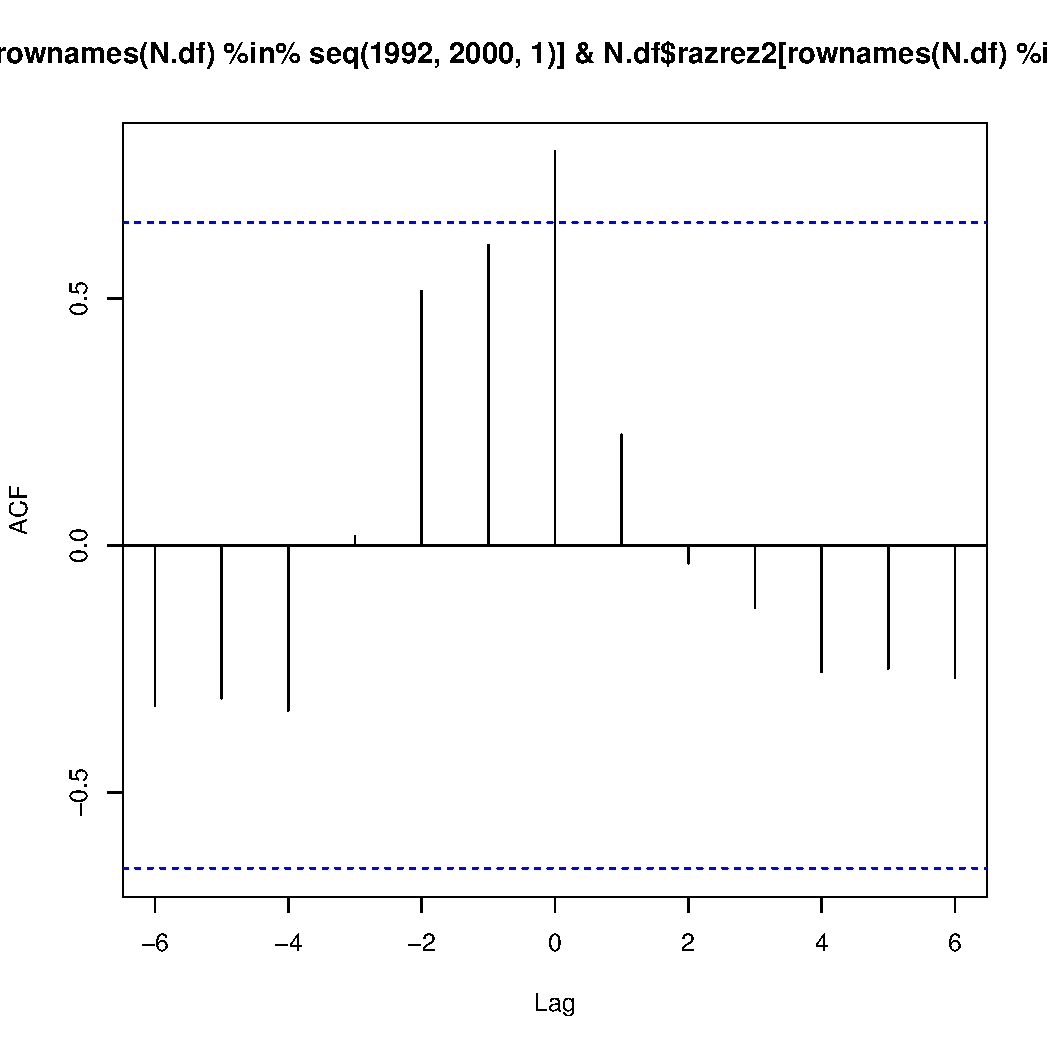
\includegraphics[width=65mm]{../White_Sea/dynamic_N_N1/crosscorr_N_Seldyanaya_2razrez_1992_2000.pdf}
	\end{center}
	\end{minipage}
%
	\hfil %Это пружинка отодвигающая рисунки друг от друга
%
	\begin{minipage}[b]{.46\linewidth}
%Следующий рисунок - первый ряд справа %DUNGEON S_4 \ AB
	\begin{center}
	{\tiny   N Medvezhya 2razrez 1992 2000}
	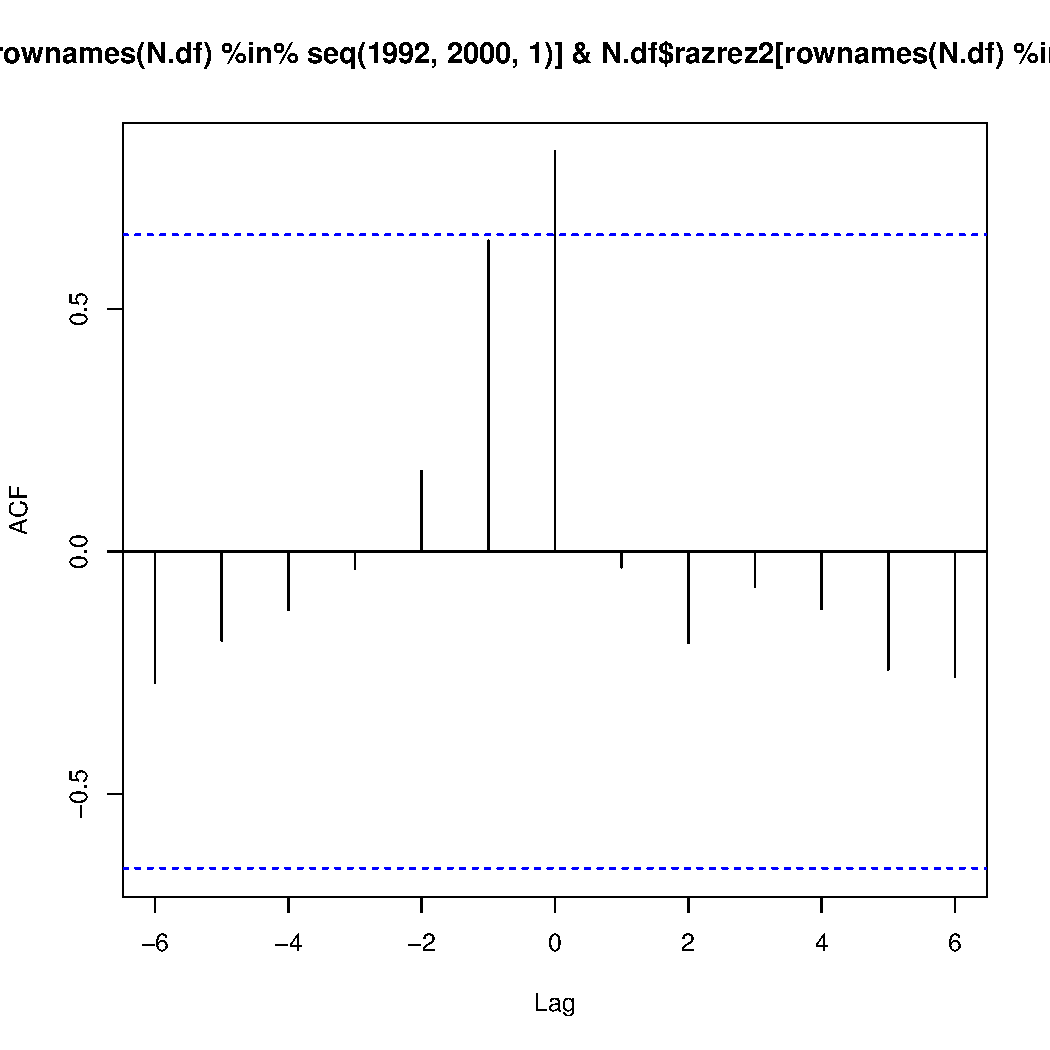
\includegraphics[width=65mm]{../White_Sea/dynamic_N_N1/crosscorr_N_Medvezhya_2razrez_1992_2000.pdf}
	\end{center}
	\end{minipage}

%\smallskip
%	\caption{Динамика плотности поселений {\it Macoma balthica} в вершине Кандалакшского залива}
%	\label{ris:dynamic_Kandalaksha_all}
\begin{center}
Рисунок \ref{ris:сcrosscorr_N_Kandalaksha}, продолжение. Кросскорреляции средней численности {\it Macoma balthica} на разных в Кандалакшском заливе
\end{center}
	\end{figure}

	\begin{figure}[ht]
	
	\begin{minipage}[b]{.46\linewidth}
	%Фигурка в первом ряду слева размер отведенный под весь этот объект \textendash 0.46 от ширины строки
	%Параметр [b] означает, что выравнивание этих министраниц будет по нижнему краю
	\begin{center}
	{\tiny  N Seldyanaya ZRS 1994 2012}
		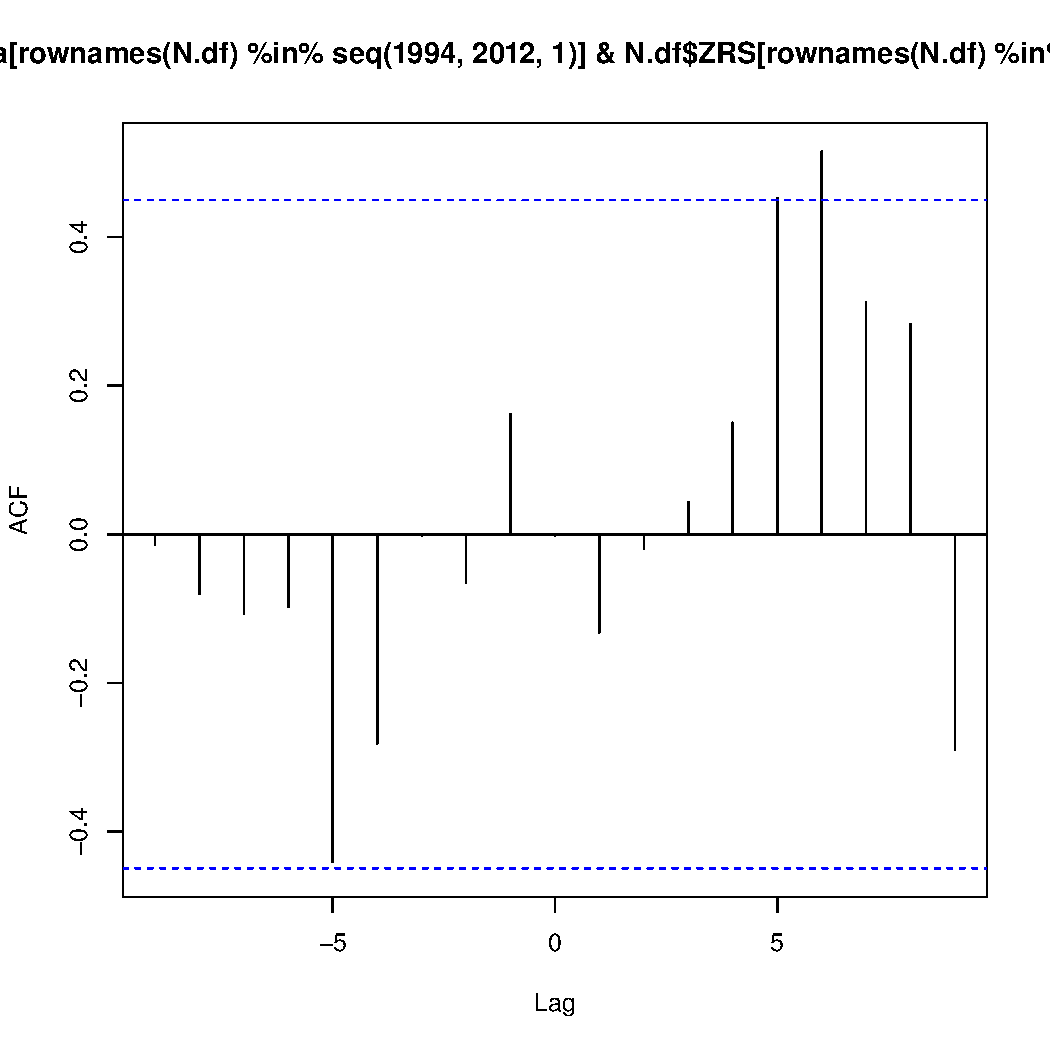
\includegraphics[width=65mm]{../White_Sea/dynamic_N_N1/crosscorr_N_Seldyanaya_ZRS_1994_2012.pdf}

	\end{center}
	\end{minipage}
	%
	\hfil %Это пружинка отодвигающая рисунки друг от друга
	%
	\begin{minipage}[b]{.46\linewidth}
%Следующий рисунок - первый ряд справа %DUNGEON S_4 \ AB
	\begin{center}
	{\tiny   N Medvezhya ZRS 1994 2012}
		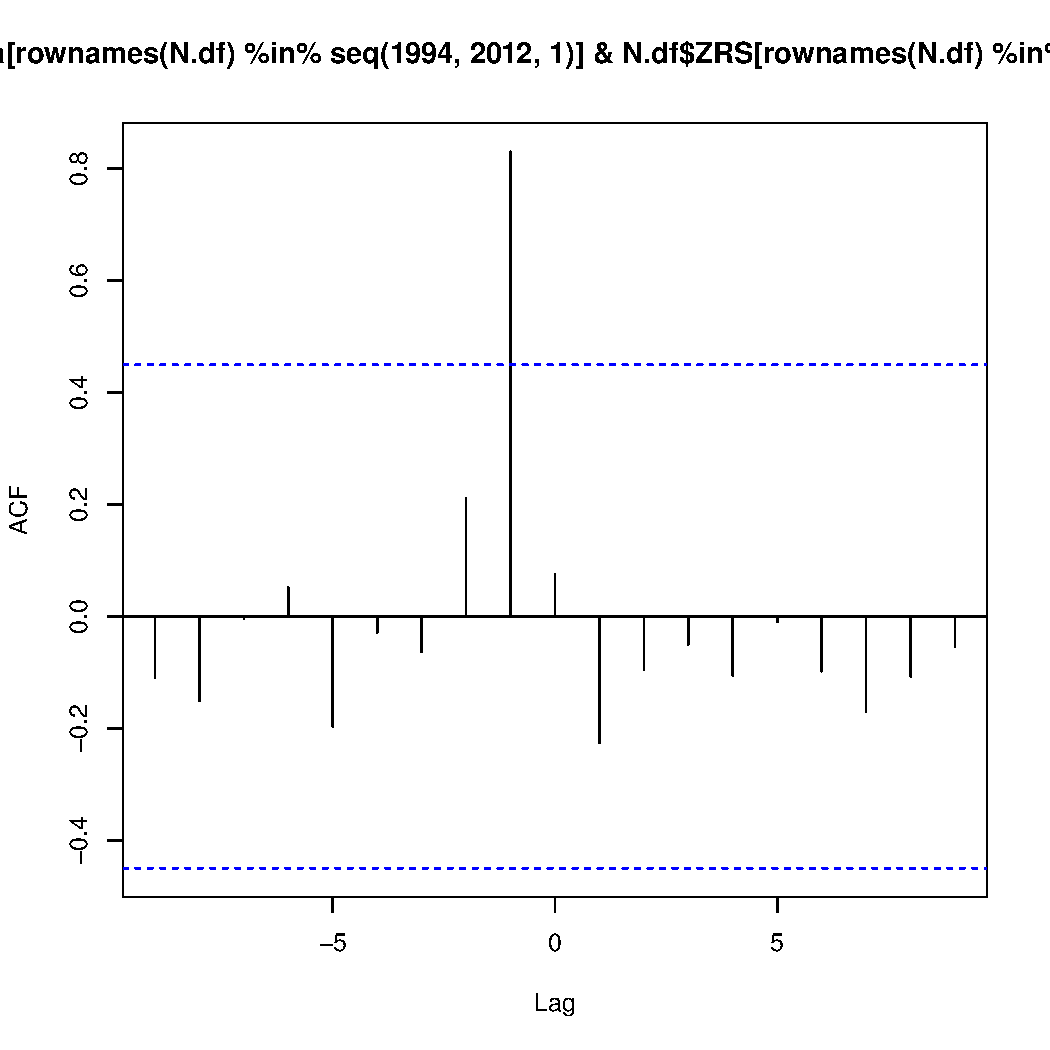
\includegraphics[width=65mm]{../White_Sea/dynamic_N_N1/crosscorr_N_Medvezhya_ZRS_1994_2012.pdf}
	\end{center}
	\end{minipage}

%\smallskip


%
	\begin{minipage}[b]{.46\linewidth}
%Следующий рисунок - первый ряд справа %DUNGEON S_4 \ AB
	\begin{center}	
	{\tiny   N ZRS 2razrez 1994 2000}
	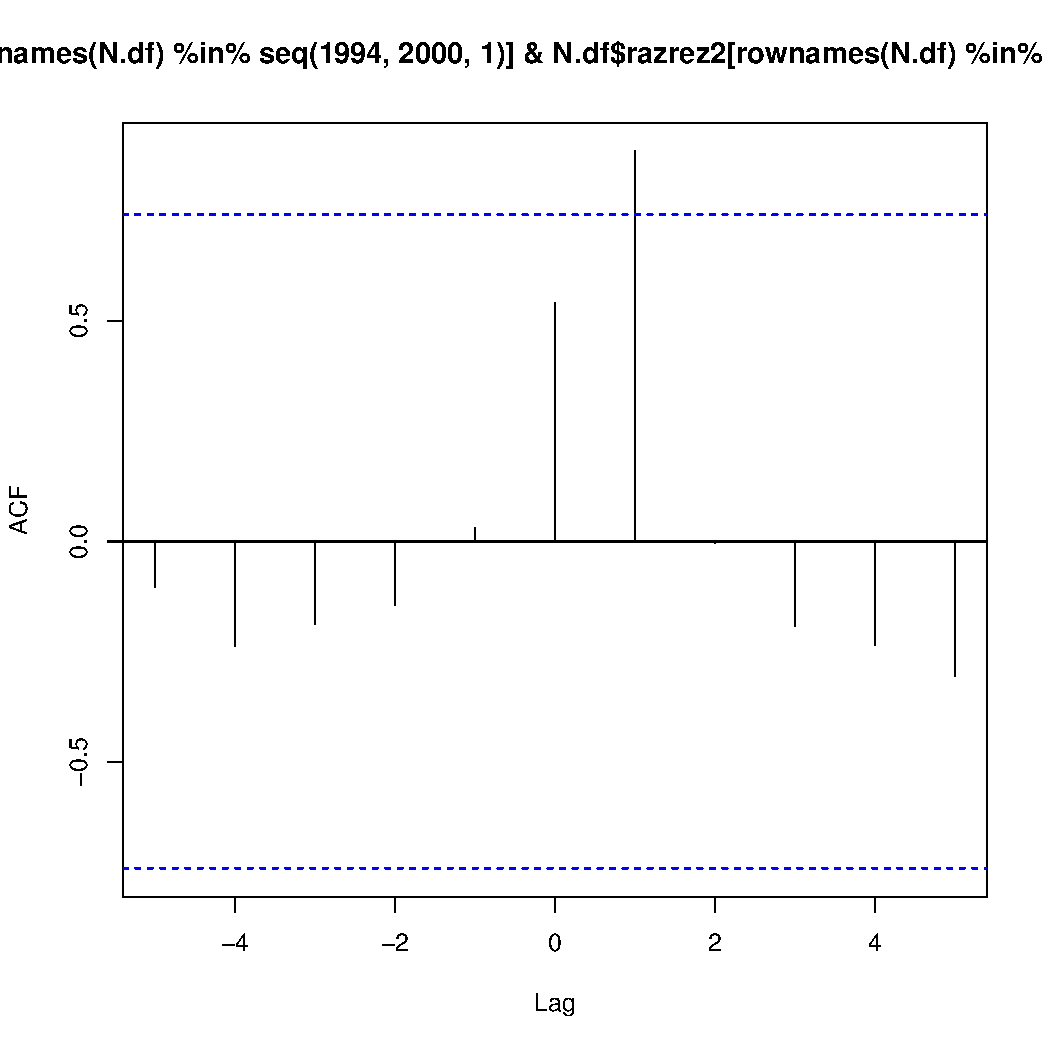
\includegraphics[width=65mm]{../White_Sea/dynamic_N_N1/crosscorr_N_ZRS_2razrez_1994_2000.pdf}
	\end{center}
	\end{minipage}
\hfil %Это пружинка отодвигающая рисунки друг от друга
	\begin{minipage}[b]{.46\linewidth}
%Фигурка в первом ряду слева размер отведенный под весь этот объект \textendash 0.46 от ширины строки
%Параметр [b] означает, что выравнивание этих министраниц будет по нижнему краю
	\begin{center}
	{\tiny  N Medvezhya Seldyanaya 1987 2013}
	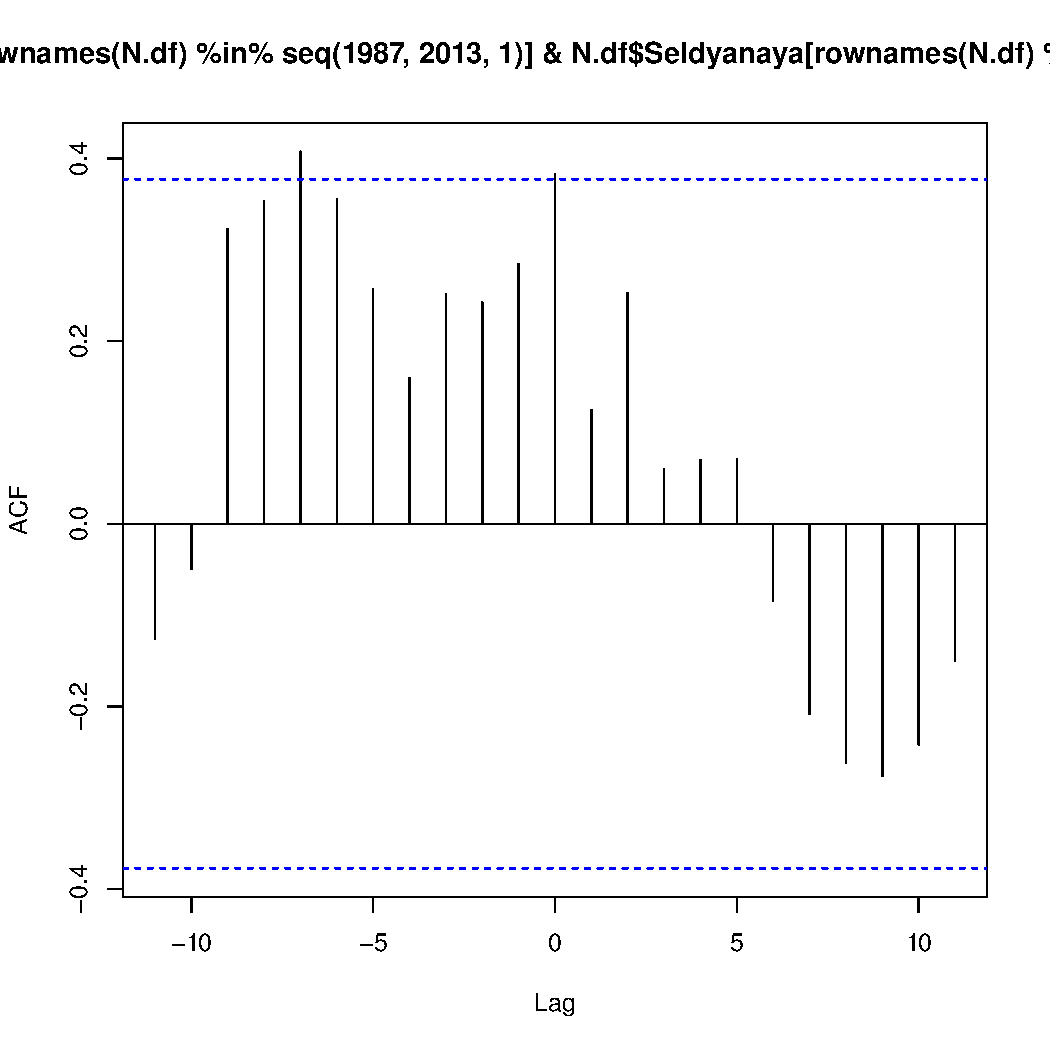
\includegraphics[width=65mm]{../White_Sea/dynamic_N_N1/crosscorr_N_Medvezhya_Seldyanaya_1987_2013.pdf}
	\end{center}
	\end{minipage}
%
%	\hfil %Это пружинка отодвигающая рисунки друг от друга
%
%	\begin{minipage}[b]{.46\linewidth}
%Следующий рисунок - первый ряд справа %DUNGEON S_4 \ AB
%	\begin{center}
%	{\tiny 2 разрез верхний пляж}
%	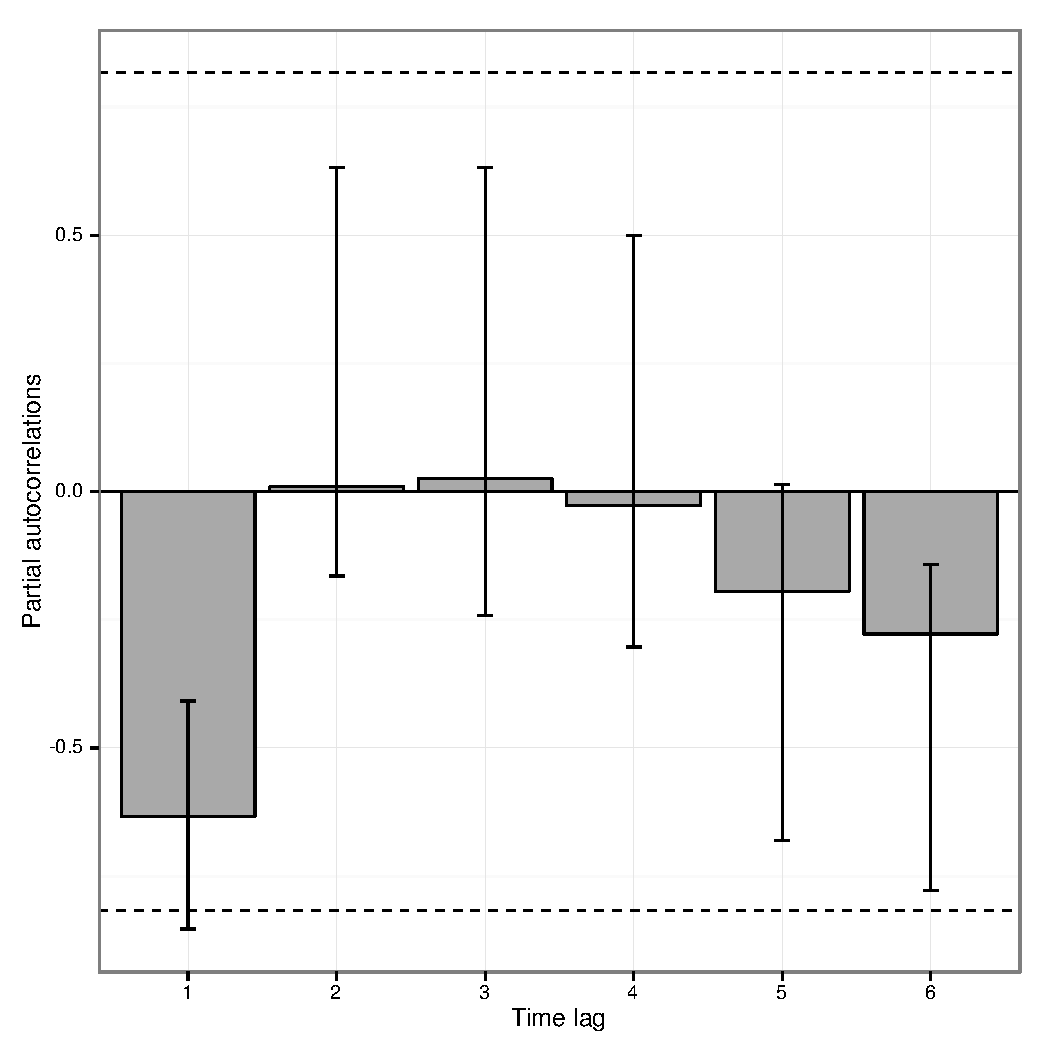
\includegraphics[width=65mm]{../White_Sea/dynamic_N_N1/boot_PRCF_razrez2_high_beatch_.pdf}
%	\end{center}
%	\end{minipage}

%\smallskip
	\begin{center}
Рисунок \ref{ris:сcrosscorr_N_Kandalaksha}, продолжение. Кросскорреляции средней численности {\it Macoma balthica} на разных в Кандалакшском заливе
\end{center}
	\end{figure}


\end{document}
